\documentclass{article}
\usepackage[utf8]{inputenc}
\usepackage[spanish]{babel}
\usepackage{listings}
\usepackage{graphicx}
\graphicspath{ {images/} }
\usepackage{cite}

\begin{document}

\begin{titlepage}
    \begin{center}
        \vspace*{1cm}
            
        \Huge
        \textbf{Ideación Nro 2}
            
        \vspace{0.5cm}
        \LARGE
        Proyecto final Informática II \\
        Video juego: Dot
            
        \vspace{1.5cm}
            
        \textbf{Miguel H. Martin Matiz}
            
        \vfill
            
        \vspace{0.8cm}
            
        \Large
        Despartamento de Ingeniería Electrónica y Telecomunicaciones\\
        Universidad de Antioquia\\
        Medellín\\
        16 de Septiembre de 2021
            
    \end{center}
\end{titlepage}

\tableofcontents
\newpage
\section{Introducción}\label{intro}

\textbf{Dot} es un juego con un enfoque minimalista y de tipo lógica recreado en un escenario donde los obstáculos son figuras geométricas básicas con 0, 1 y 2 dimensiones, desde la más simple como un punto, lineas rectas y curvas hasta las más complejas (en cuanto a lados), como triángulos, cuadrados, pentágonos, hexágonos y más. Un punto es el personaje principal, por supuesto llamado Dot. A lo largo del juego, Dot se encontrará con distintos obstácuos que el usuario deberá superar para avanzar resolviendo el desafío que se propone en cada estación.
\\
\section{Descripción del proyecto} \label{imagenes}
El juego se desarrollará en formato plataforma, ambientando por figuras geométricas de máximo 2 dimensiones, siendo un punto el personaje principal que recorrerá los escenarios. Para poder visualizar bien en pantalla al punto, se hará por supuesto más grande que un punto de un pixel. La dificultad para el jugador en cada escenario será resolver el obstáculo propuesto, haciendo uso de los elementos presentes para construir distintos mecanismos o idear estrategias que le permitan avanzar. Nuestro personaje podrá rodar y saltar hasta cierta altura. Al jugador se le darán pistas que le permitan encontrar la solución.

\subsection{Escenarios}
\subsubsection{Escenario 1: } \label{EarthOrbit}
En este escenario tenemos los elementos A (Dot), B (botón), C (línea plegable) y D (línea móvil). C estará suspendido en el aire. Para superar este escenario, Dot debe saltar y golpear ambos bordes de la línea C hasta darle forma de caja como en el frame 6 de la figura (\ref{fig:escenario1}). Una vez formada la caja, que estará inmóvil en el aire, Dot debe saltar encima del botón para hacer caer la caja y luego empujarla hasta dejarla debajo de la línea D. Esta línea se estará moviendo constantemente de izquierda a derecha y viceversa sobre el mismo punto. El objetivo en este escenario será poner la caja debajo de la línea D, de forma que la línea (con el peso) la inserte en el suelo y Dot pueda meterse en el espacio que se genera debajo del suelo (como en el frame 13) para luego cruzar al otro lado donde pivota la línea D. Dot debe evitar tocar esta línea, de lo contrario morirá.
\\\\
\textbf{Pista para el jugador: }Quizá la linea que flota puede ser más útil debajo del suelo. Quizá la estrategia del avestruz pueda servirte para no morir en el intento.

\begin{figure}[h]
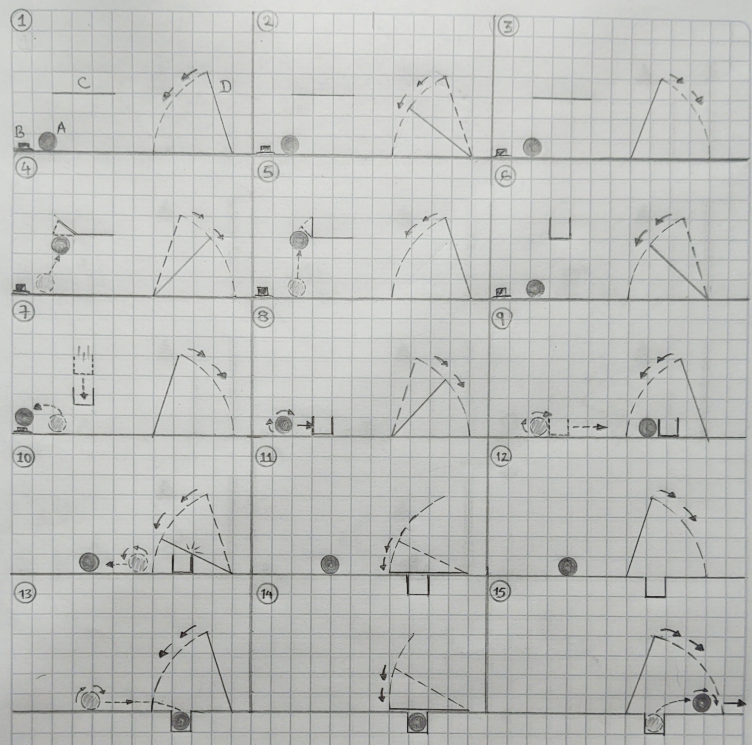
\includegraphics[width=12cm]{escenario1.png}
\centering
\caption{ Escenario donde Dot debe esconderse en el suelo para no ser aplastado y poder cruzar el obstáculo. }
\label{fig:escenario1}
\end{figure}
\subsubsection{Escenario 2:}
En este otro escenario tenemos los elementos A (Dot), B (botón), C (línea plegable), D (barra de equilibrio), E (contrapeso) y F (obstáculo fijo). El objetivo será plegar la línea C nuevamente en una caja, luego accionar el botón para que caiga y golpearla en los lados para formar un triángulo, que será el punto de equilibrio donde se posará la barra. Dot debe mover el triángulo (punto de equilibrio) hasta la marca y luego accionar de nuevo el botón para dejar caer la barra D sobre el triángulo, como en el frame 9 de la figura (\ref{fig:escenario2}). Una vez la barra esté inclinada hacia el lado izquierdo, Dot debe accionar por última vez el botón y solo en ese momento tendrá 3 segundos para posicionarse sobre el extremo izquiedo de la barra y esperar a que caiga sobra el extremo derecho el triángulo sombreado (contrapeso) para así lanzarse como en catapulta sobre el obstáculo F.
\\\\
\textbf{Pista para el jugador: } No olvides lo útil que fue la línea que flota, pero esta vez no te fíes del avestruz. Quizá Pitágoras pueda echarte una manito o quizá un brazo bien equilibrado. A lo mejor el avestruz pueda volar.

\begin{figure}[h]
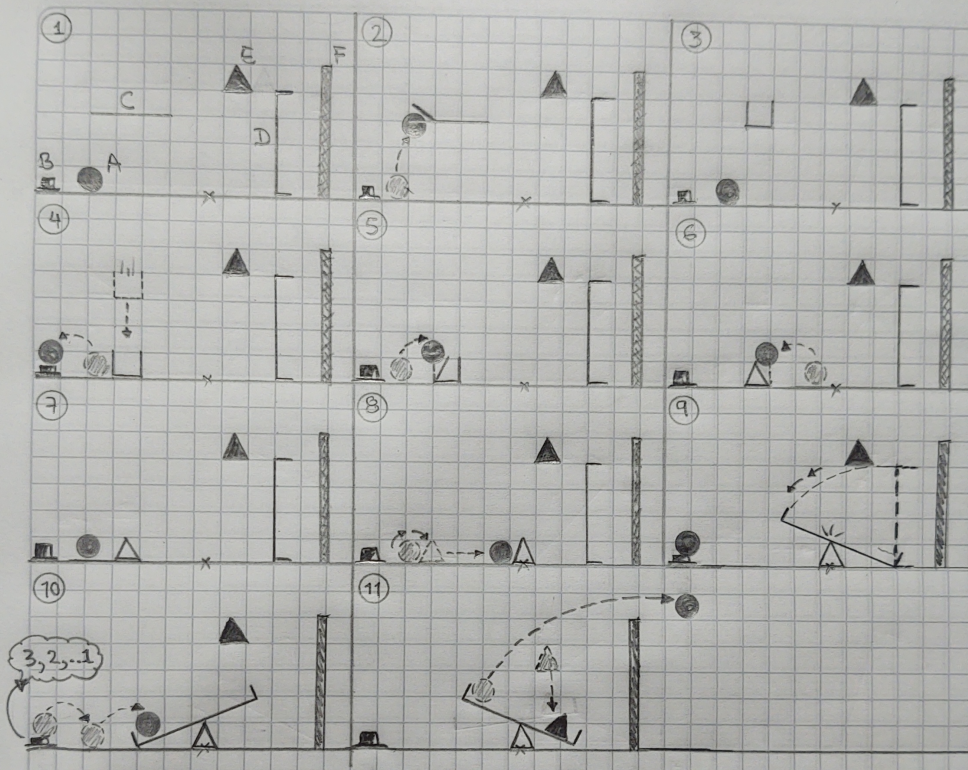
\includegraphics[width=12cm]{escenario2.png}
\centering
\caption{Dot es lanzado como en catapulta sobre el obstáculo.}
\label{fig:escenario2}
\end{figure}


\clearpage
\bibliographystyle{IEEEtran}
\bibliography{references}

\end{document}
